\section{Schedule}

\subsection{Gantt Chart}
% The initial task break-down schedule displayed graphically as a Gantt chart.
% (see https://www.fool.com/the-blueprint/gantt-chart/)
% Gnatt charts list the tasks, show the length of each task, and dependencies
% between tasks.  

We went with the agile method here. Time indications show number of weeks.  
\begin{figure}[!htb]
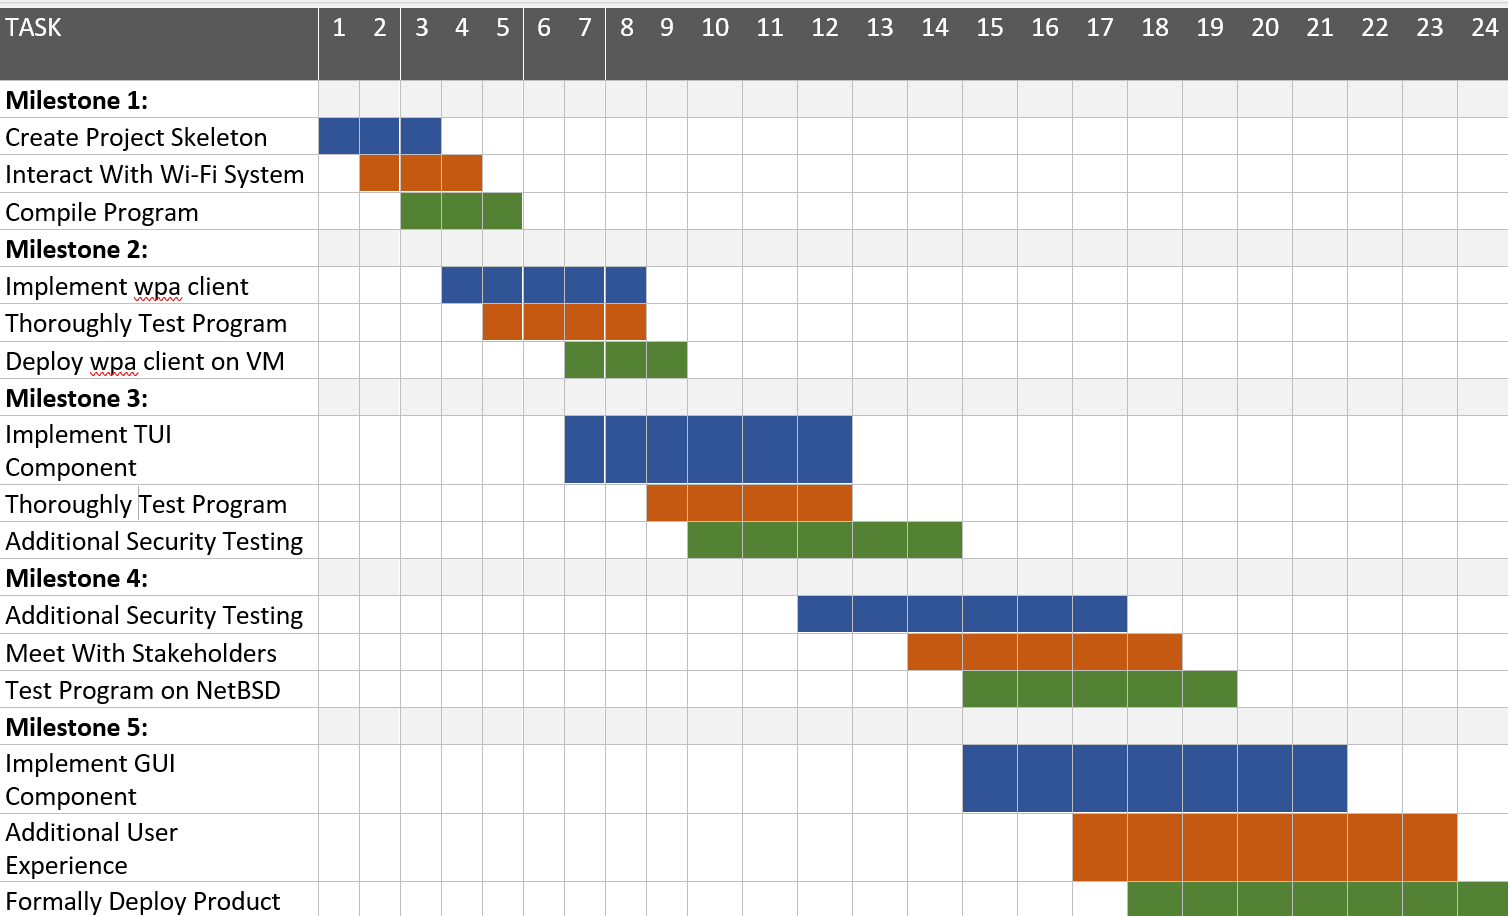
\includegraphics[scale=0.40]{ganttChart.png}
\end{figure}

\subsection{Key Milestones}
% Milestones are points in the development where you have implemented some
% number of major features.  For senior project, you generally have five
% milestones: one at the end of 491, three in 492, and one in 493.
% In this section, divide the Major Features between the milestones.  You should
% front-load the schedule as much as possible.  That is, leave 10% of the work
% for the last milestone.  

Milestone 1: Create skeleton of project. Skeleton will include any methods we think will help in creating our project. Will also contain header 
files that will link all files together, as well as a makefile to make an executable of our project. For our skeleton to be successful, we will 
need to make sure we are interacting with the system of NetBSD that is responsible for connecting to Wi-Fi, as well as streamlining the process 
through wpa\_client. For milestone one, we are only interested in setting up the proper procedures to interact with NetBSD and wpa\_client with minimal 
functionality. 

Milestone 2: Ensure product is working correctly. With our implementation and skeleton files ready, we can start to create the proper methods and procedures 
needed to make sure our system is secure. Set up additional methods to connect to Wi-Fi through wpa\_client. 

Milestone 3: Thoroughly test project to make sure it is working properly. Begin development on TUI that will interact with our system. Focus on software security 
as well as efficiency during milestone 3. 

Milestone 4: Begin development of GUI to interact with our system. Meet with stakeholders as needed. Thoroughly test product on virtual machine to ensure it works 
correctly and streamlines the process of connecting to Wi-Fi. 

Milestone 5: Meet with additional stakeholders at the time of deployment. Look for vulnerabilities in software and how to mitigate each vulnerability. Clean up any 
additional code and ensure product is working correctly. 


\subsection{Resource Assignments}
% Resources include budgets, consumables like paint, and computing equipment
% like servers and development systems.  Assign these resources, if any, to the
% tasks, listed above. 
%

Resources will include Western computers that can interact with NetBSD operating system so we can test our product. Additional resources will include 
additional computers to work on developing our project. Budgets and additional consumables I don’t think are needed here. 


\subsection{Individual Responsibilities}
% Who is responsible for which parts of the development effort.
%
Stephen Loudiana - Responsible for completing work not done on campus (stakeholders / writing)
Kevin / Dylan - Split responsibilities for working on campus (interacting with vm, etc.) 

